\documentclass{elsart}  
\usepackage{epsfig,amssymb,amsmath}  
\begin{document}


\section{Drift velocity and gas gain}

As shown in the Langevin equation \cite{blum}[p.49], the drift velocity is a function of the field (electric, magnetic) and the mobility. The mobility depends on the gas density which is a function of the environment variables as well as the gas composition which can change in time. 

$$v_d = v_d(E/N) = v_d(E,B,T,P,C_{CO_2},C_{N_2})$$

$E$ and $B$ are the field values (electric, magnetic), $N$ is the gas density, $P$ is the atmospheric pressure, $T$ is the temperature inside of the TPC and $C_{CO_2}$ and $C_{N_2}$ are two concentration out of three components of the drift gras $Ne,CO_2,N_2$ (90/10/5) within the TPC. We suppose that these parameters, especially the environment variables, will vary in time within a reasonable range. However, according to performed \textsl{Magboltz-2} \cite{magboltz} simulations a first order Taylor expansion of the dependencies around the nominal values is sufficient. More details can be found in section \ref{sec:magbolzSim}.
\begin{equation}
\Delta{v_d}=v_d-v_{d0}=\frac{dv}{dE}\Delta{E}+\frac{dv}{dN}\Delta{N(P,T)}+\frac{dv}{dC_{CO_2}}\Delta{C_{CO_2}}+\frac{dv}{dC_{N_2}}\Delta{C_{N_2}}
\label{equ:taylor}
\end{equation}

Within the TPC volume, the parameters in the expansion are changing with different time constant. A significant change of the drift velocity due to the gas composition changes has a time constant of days. On the other hand the changes due to the pressure and temperature variation have to be corrected on the level of minutes.
In the following we will focus on the influence of the changes of the gas density, temperature and pressure. 
\begin{equation}
\frac{\Delta{v_d}}{v_{d0}}= k_t(t)+k_{N}\frac{\Delta{N(P,T)}}{N_0(P,T)} 
\end{equation}
\begin{equation}
\frac{\Delta{v_d}}{v_{d0}}= k_t(t)+k_{P/T}\frac{\Delta{(P/T)}}{(P/T)_0} 
\end{equation}

The factor of the time dependent offset $k_t(t)$ describes then the influence of the gas composition and possible changes within the field. 

The correction factor $v_c=\frac{\Delta{v_d}}{v_{d0}}$ can be measured using different methods:
\begin{itemize}
\item Matching laser tracks with the surveyed mirror position
\item Matching with the ITS tracks
\item Matching of the TPC primary vertices from the two halves of the TPC
\item Using cosmic tracks - matching tracks from two halves of the TPC
\end{itemize}

The unknown parameters $k_t(t)$ and $k_N$ can be than fitted using the Kalman filter as is shown in section \ref{sec:kalman}.


\section{Simulation of drift velocity dependencies }
\label{sec:magbolzSim}

The state-of-the-art program \textsl{Magboltz-2} \cite{magboltz} can be used to calculate different drift properties by means of MonteCarlo (MC) methods as for example the drift velocity within a certain gas mixtures, under certain environment conditions and with any choosen field. Since MC simulations itself are too time consuming, a first order tayler expansion was used in order to fit various simulated data points under different conditions. Upper and lower tresholds for the simulated points were choosen to be within a reasonable range of possible changes within the TPC as shown in table \ref{tab:valRange}.  This approximation was implemented within the class \textsl{AliTPCCalibVDrift}. It allows to estimate the drift velocity, as a function of field and gas properties changes, quickly and with sufficient accuracy, at least for a first order calibration.\\

\begin{table}[htbp]
\caption{Dependency range of simulated drift velocities}
\centering
\begin{tabular}{|l|r|r|r|}
\hline
 & \multicolumn{1}{l|}{std.cond.} & \multicolumn{1}{l|}{MIN} & \multicolumn{1}{l|}{MAX}  \\ \hline
E [V/cm] & 400 & 395 & 405 \\ \hline
T [K]& 293 & 288 & 300  \\ \hline
P [TORR]& 744 & 719 & 759 \\ \hline
Co2 [\%]& 9.52 & 9.02 & 10.02  \\ \hline
N2 [\%]& 4.76 & 4.36 & 5.26  \\ \hline
\end{tabular}
\label{tab:valRange}
\end{table}


The following dependencies were obtained through fitting the simulated $v_d$'s with a linear hyperplane which is equal to the first order taylor expansion from equation (\ref{equ:taylor}). 

\begin{eqnarray*}
  \frac{\partial v_d}{\partial E} & = & 0.24 \; [cm/V\mu s] \\
  \frac{\partial v_d}{\partial T} & = & 0.31 \; [cm/K\; \mu s]\\
  \frac{\partial v_d}{\partial P} & = & -0.13 \; [cm/Torr\; \mu s]\\
  \frac{\partial v_d}{\partial C_{CO_2}} & = & -6.60 \; [cm/\%\; \mu s]\\
  \frac{\partial v_d}{\partial C_{N_2}} & = & -1.73 \;[cm/\%\; \mu s]
\end{eqnarray*}


Two example plots are given in figure \ref{figVDdepend} where the drift velocity change is plotted in dependency of pressure and temperature. A residual histogram of the complete taylor expansion with all dependencies is plotted in figure \ref{figResHistoSim}. The sigma of the residual distribution is lower than the claimed relative precision of \textsl{Magboltz-2}, which is 0.05\%. This proves that the first order taylor approximation is valid within the chosen range of possible variations.


\begin{figure}[t]
\centering
\includegraphics[width=0.48\textwidth]{picDCS/NeCO2N2_T-vd.epsi}
\includegraphics[width=0.48\textwidth]{picDCS/NeCO2N2_P-vd.epsi}
\caption{
Change of drift velocity in dependency of temperature (left) and pressure (right). } 
\label{figVDdepend}
\end{figure}

\begin{figure}[t]
\centering
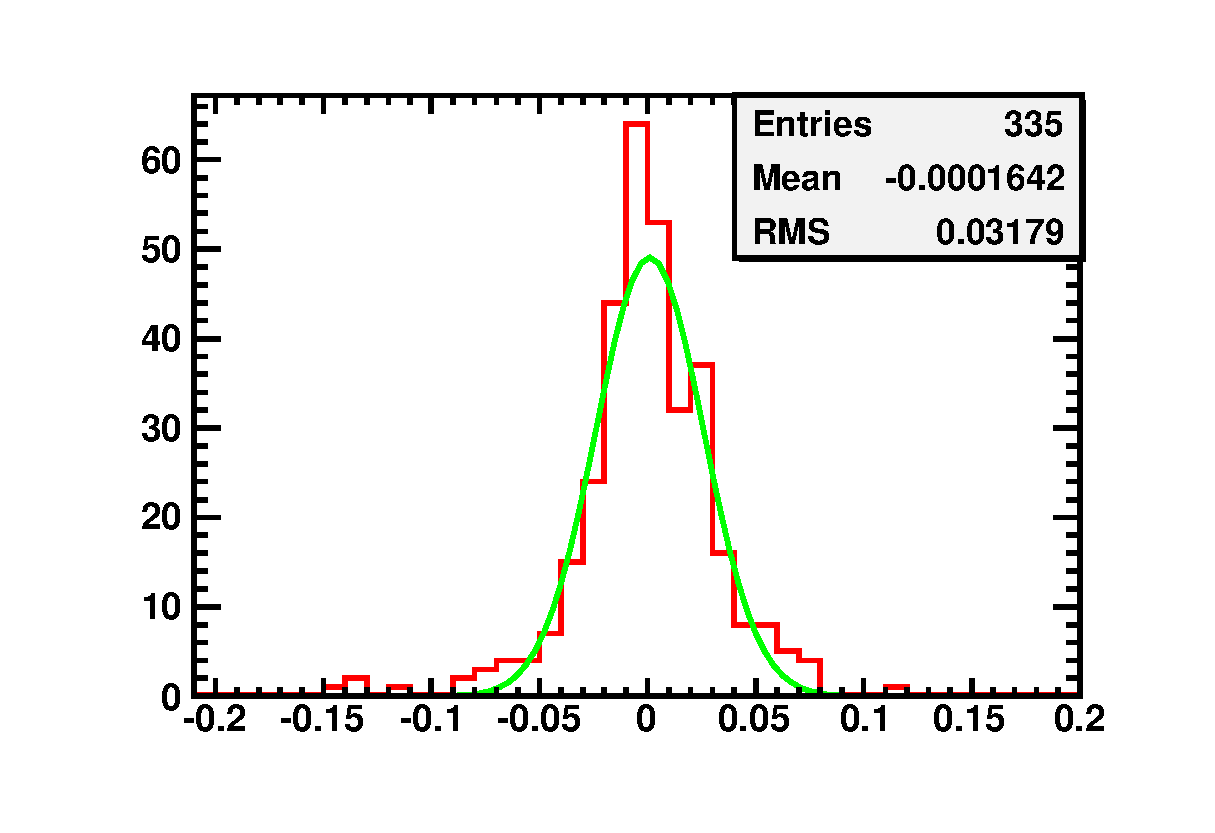
\includegraphics[width=90mm]{picDCS/resHist.eps}
\caption{
Fit residuals of drift velocity change in [\%]. } 
\label{figResHistoSim}
\end{figure}



\section{Kalman filter for time dependent variables}
\label{sec:kalman}
The drift velocity and the gas gain are changing in time.
The drift velocity and gas gain is a function of many parameters, but not all of 
them are known. We assume that the most important parameters are pressure and temperature
and the influence of other parameters (gas composition, and electric field) are only 
slowly varying in time and can be expressed by smooth function $x_{off}(t)$:
\begin{equation}
x(t) = x_{off}(t)+k_N\frac{\Delta{P/T}}{P/T}
\label{eq:KalmanTime}	
\end{equation}
where x(t) is the parameter which we observe.
\begin{equation}
\begin{split}
x(t)=\frac{\Delta{G}}{G_0}	\\
x(t)=\frac{\Delta{v_d}}{v_{d0}}	
\end{split}
\end{equation}

The Kalman filter parameters are:
\begin{itemize}
\item State vector  ($x_{off}(t)$, $k_N$) at given time
\item Covariance matrix
\end{itemize}

The Kalman filter implement the following functions:
\begin{itemize}
\item Prediction - adding covariance element $\sigma_{xoff}$
\item Update state vector with new measurement vector ($x_t,\frac{\Delta{P/T}}{P/T}$)
\end{itemize}

\begin{figure}[t]
\centering
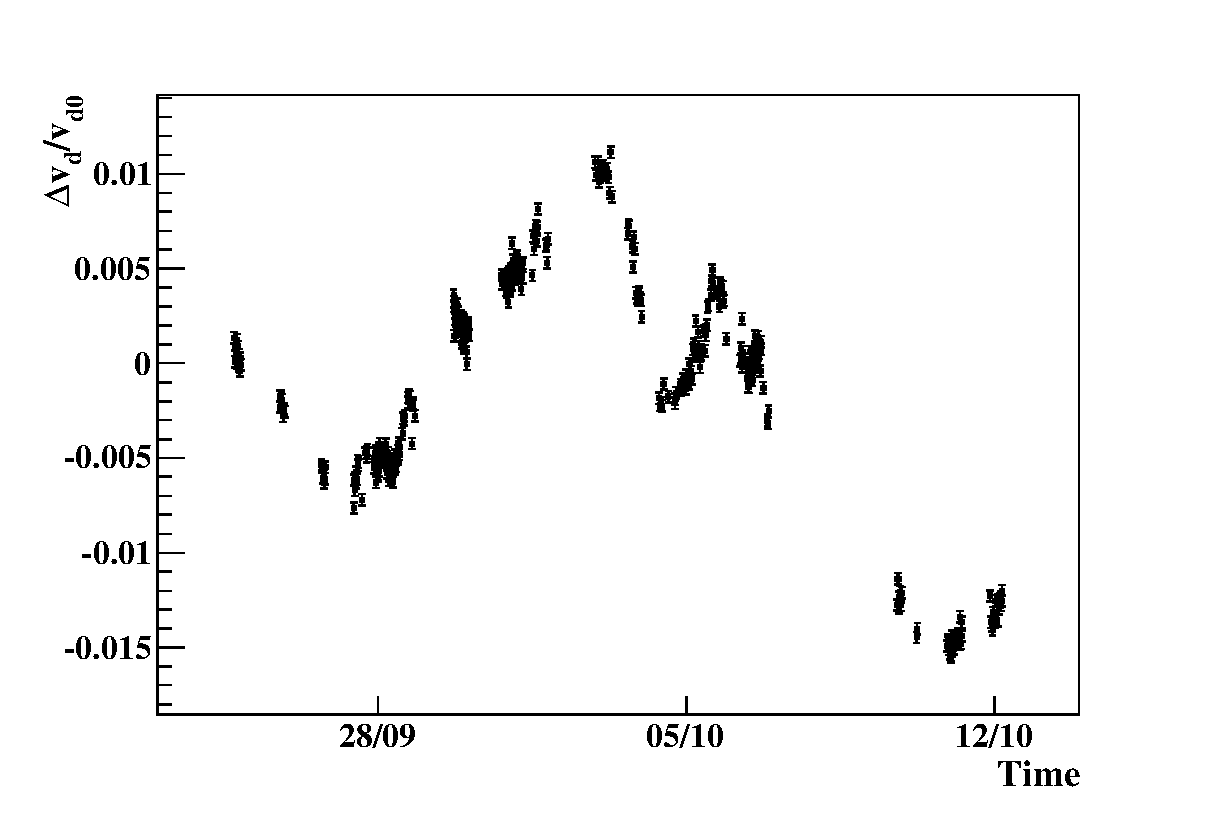
\includegraphics[width=80mm]{picDCS/vdriftraw_time.eps}
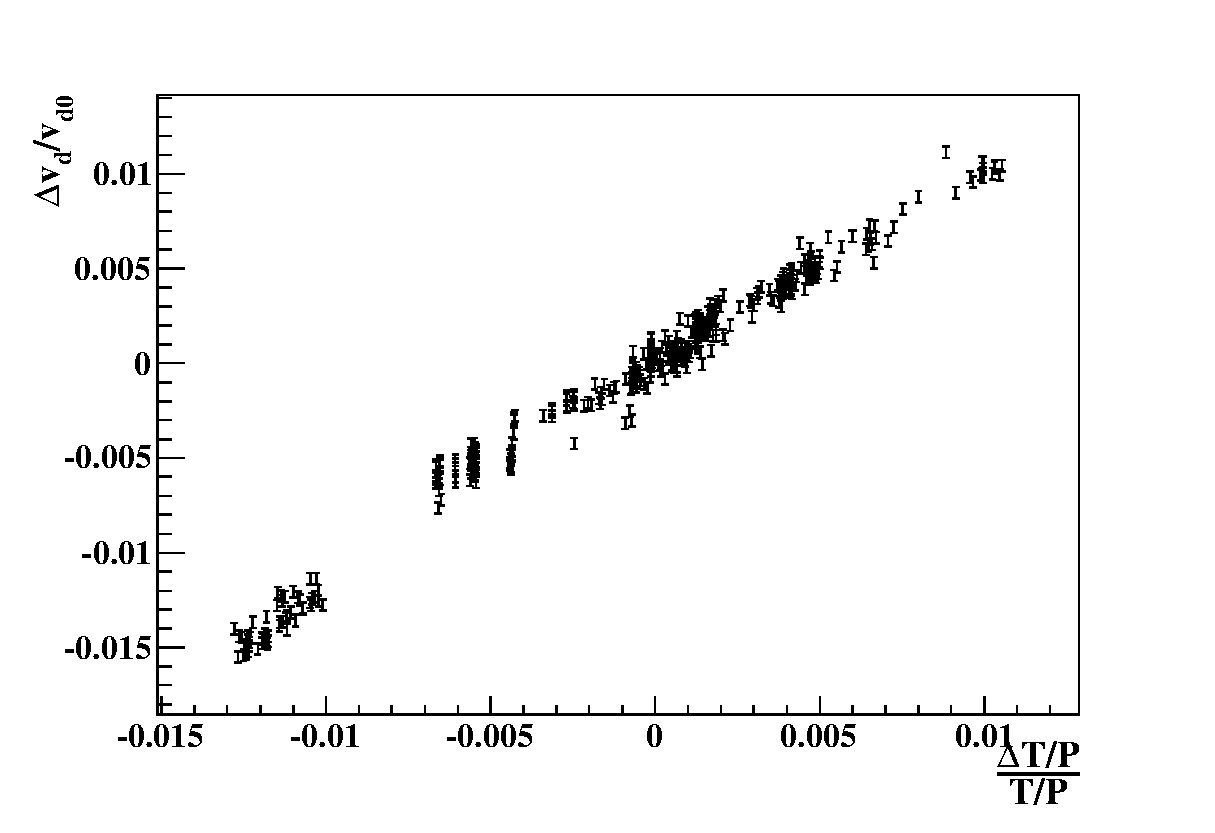
\includegraphics[width=80mm]{picDCS/tpraw_tp.eps}
\caption{
	Drift velocity as function of time (upper plot) and as a function of $\Delta(T/P)$ (lower plot)
} 
\label{figVDrift}
\end{figure}

\begin{figure}[t]
\centering
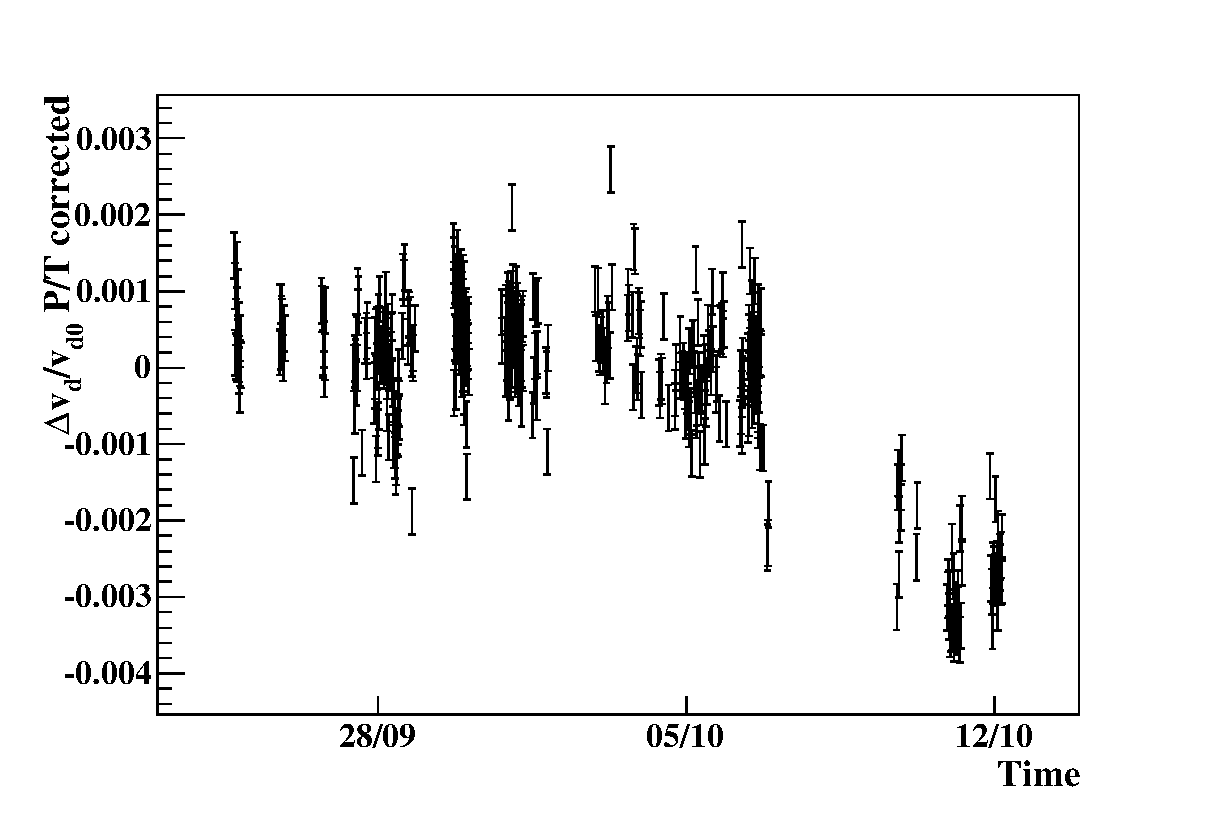
\includegraphics[width=80mm]{picDCS/vdriftptcorr_time.eps}
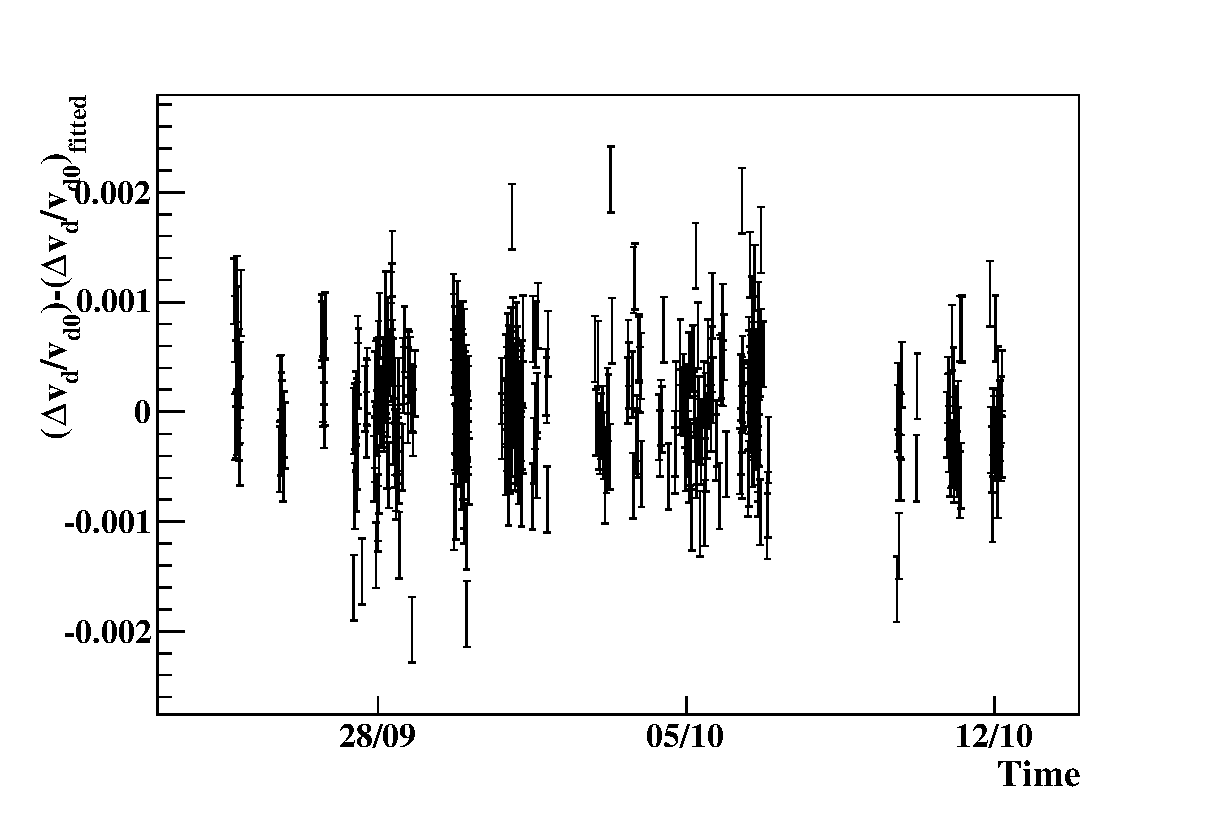
\includegraphics[width=80mm]{picDCS/vdriftfdrift_time.eps}
\caption{
	Drift velocity corrected for T/P variation as function of time (upper plot). 
	In the lower plot the correction for time dependent offset is  also applied ($x_{off}(t)$ in formula\ref {eq:KalmanTime})
} 
\label{figVDriftCorrected}
\end{figure}





\section{Precision of the correction}

The precision of the drift velocity correction and gain correction is proportional
to the  precision of the pressure and temperature measurement and to the length of the time
interval 
\begin{eqnarray}
    \sigma^2_x=\sigma^2_{xoff}\Delta{t}+k^2_N\sigma^2_{P/T}
\label{eq:sigmaX}
\end{eqnarray}

The typical relative resolution of the pressure and temperature measurement is on the level of $6\times10^{-5}$ and
$1\times10^{-5}$ respectively (see picture \ref{figDCSResol}). For cool gas the  coefficient $k_N$ is close to one. The contribution of the P/T correction to the drift velocity uncertainty is on the level of  $6.1\times10^{-5}$ (150 microns for the full drift length of 250 cm)

The $\sigma_{xoff}$ from equation \ref{eq:sigmaX} was  estimated from plot \ref{figVDriftCorrected} and is on the level of 0.001 in a four day period. This estimate was obtained for the period of largest change in the present data sample. Further investigations should be carried out for extended time periods.

For the TPC drift velocity determination, the requiered relative resolution is on the level of $6\times10^{-5}$.
Entering the observed sigmas into equation (\ref{eq:sigmaX}) the minimal frequncy of the drift velocity updates were estimated (equation \ref{eq:driftUpdateTime}) to be about 1 hour.  
\begin{eqnarray}
    \Delta{t}\le\frac{\sigma^2_x}{\sigma^2_{xoff}}\approx\left(\frac{6\times10^{-5}}{0.001/4days}\right)^2=0.05 day.
\label{eq:driftUpdateTime}
\end{eqnarray}


\begin{figure}[t]
\centering
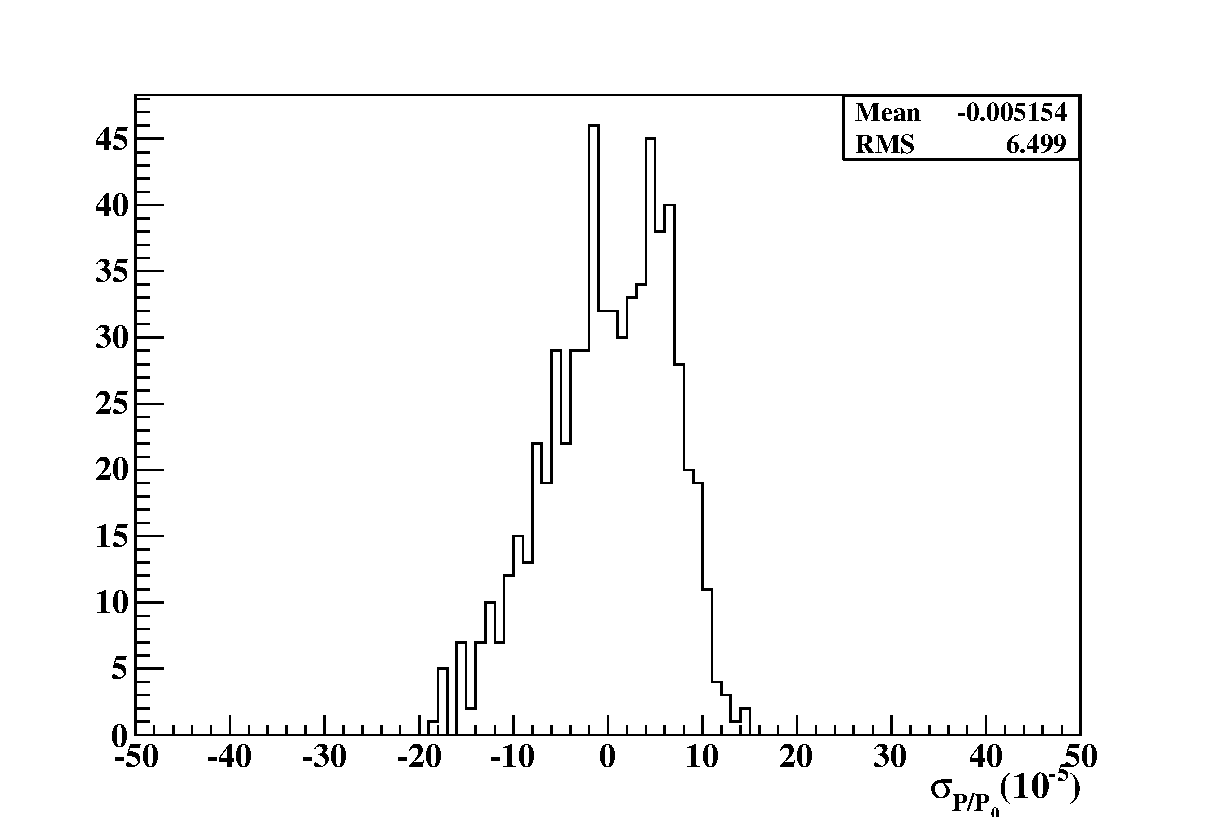
\includegraphics[width=80mm]{picDCS/deltaPoverP.eps}
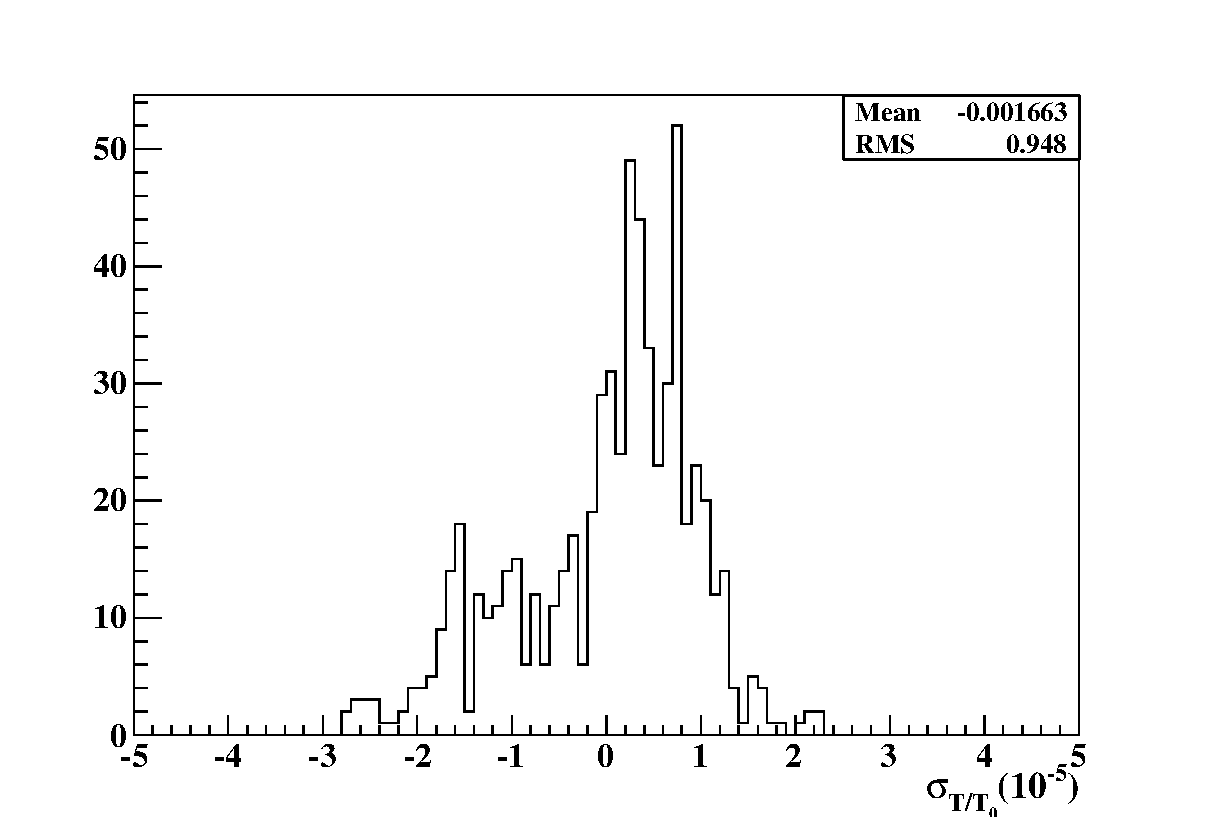
\includegraphics[width=80mm]{picDCS/deltaToverT.eps}
\caption{
The relative resolution of the pressure and temperature  measurement.
} 
\label{figDCSResol}
\end{figure}



\section{ Alice TPC drift calibration using tracks}

In the first approximation there is a linear dependence of the z position on the drift time.
In the Alice TPC the expression on the A side and C side of the chambers have the same drift velocity part $v_d$ 
with opposite sign. The full drift length $z_{0A}$ and $z_{0C}$ are different. We suppose that
the $t_0$ offset given by trigger arrival time is the same. In reality the $t_0$ equalization is applied before,
using the pad-by-pad calibration pulser measurement. We let the variable $s$ represent the sides A and C with, with respective values $s_A=-1$ and $s_C=+1$. 
\begin{equation}
\begin{split}
z_s = z_{s0}+sv_d(t-t_0)
\end{split}
\end{equation}

Let the actual value of drift velocity $v_d$ and the time offset $t_0$ are shifted by some $\Delta$ value.
Our starting drift velocity values and time offset are $\tilde{v}_d$ and $\tilde{t}_0$
\begin{equation}
\begin{split}
v_d=\tilde{v}_d+\Delta v_d \\
t_0=\tilde{t}_0+\Delta t_0 \\
v_c = \frac{\Delta{v_d}}{\tilde{v}_d} \\
\Delta{z}_{t_0} = \Delta{t}_0\tilde{v}_d \\
\end{split}
\end{equation}

Then the actual z position is expressed using the starting z position measurement $\tilde{z}_s$. 
\begin{equation}
\begin{split}
z_s = \tilde{z}_s-\frac{\Delta v_d}{v_d}(z_{s0}-\tilde{z}_{s})-s\Delta t_0 \tilde{v}_d\\= \tilde{z}_{s} -v_c(z_{s0}-\tilde{z}_{s})+\Delta{z}\\
\end{split}
\end{equation}


In previous expression  we neglected second order correction
\begin{equation}
\begin{split}
\Delta{v_d}\Delta{t_0}\ll\frac{\Delta v_d}{v_d}(z_{s0}-z_{s}) \\
(t-t_0)\approx \frac{(z_{s0}-\tilde{z}_{s})}{v_d}
\end{split}
\end{equation}

Combining the z measurement the track parameters can be fitted. Let's assume linear track model:
\begin{equation}
\begin{split}
\tilde{z}_s =\tilde{a}_s+\tilde{b}_sx \\
z_s = a_s+ b_sx \\
\end{split}
\end{equation}

The relation between starting  parameters $\tilde{a}, \tilde{b}$ and corrected parameters $a,b$ is linear.
\begin{equation}
\begin{split}
a_s=\tilde{a}_s-v_c(z_{s0}-\tilde{a}_s)-s\Delta{z}\\
b_s=\tilde{b}_s(1+v_c)\\
\end{split}
\end{equation}
The inclination angle correction is the same on the A and C side.
 
Tracks crossing the central electrode, respectively primary tracks can be used to
monitor correction coefficients $\Delta{z}$ and $v_c$. For tracks crossing the central electrode the a and b parameters at the crossing point fitted form A and C side are the same. In case of primary tracks, the z position at r-$\phi$ DCA are also the same:
\begin{equation}
\begin{split}
a_A-a_C=0 \\
\Delta\tilde{a}(1-v_c)+2\Delta{z}-v_c(z_{0A}-z_{0C})=0 \\
\Delta\tilde{a}=\frac{v_c(z_{0A}-z_{0C})-2\Delta{z}}{1-v_c}	
\end{split}
\end{equation}

Combining information from A and C side the correction parameters, drift correction $v_c$ and offset correction $\Delta{z}$ can be fitted.

In case track crossed the central electrode the track parameters of the same track on A side and C side can be fitted.
The actual track parameters $a_A$ and $a_C$  respectivally $b_A$ and $b_C$ are the same.



\begin{thebibliography}{99}

\bibitem{Blum}
W.Blum, W.Riegler, L.Luigi: Particle Detection with drift Chambers; 2nd ed.
%@book{Blum,
%      author       = "Blum, Walter and Riegler, Werner and Rolandi, Luigi",
%      title        = "Particle Detection with drift Chambers; 2nd ed.",
%}

\bibitem{magboltz}
S.Biagi: Magboltz-2, transport of electrons in gas mixtures; http://consult.cern.ch/writeup/magboltz
%@Misc{magboltz,
%  author = {S. Biagi},
%  title = {{Magboltz-2}, Transport of electrons in gas mixtures},
%  year =  {2008},
%  annote = {Version 8.3}



 \end{thebibliography}

\end{document}
